% =============================================================
% fig_arch_graphsage_lstm.tex
% Architecture diagram: GraphSAGE-LSTM (graph-based spatial encoder)
% Compile standalone:  pdflatex fig_arch_graphsage_lstm.tex
% =============================================================
\documentclass[tikz, border=8pt]{standalone}
\usepackage{amsmath,amssymb}
\usetikzlibrary{arrows.meta, positioning, fit, backgrounds, calc}

% ---- Shared colour palette (identical across all 4 architecture figures) ----
\definecolor{cInput}{HTML}{4477AA}    % blue    - input blocks
\definecolor{cSpatial}{HTML}{8855AA}  % violet  - spatial encoder
\definecolor{cGraph}{HTML}{EE9922}    % amber   - graph components
\definecolor{cTemporal}{HTML}{229988} % teal    - temporal encoder (LSTM)
\definecolor{cOutput}{HTML}{EE6677}   % coral   - output layer
\definecolor{cMuted}{HTML}{999999}    % grey    - "not used in this variant"

% ---- Shared node / arrow styles ----
\tikzset{
  font=\sffamily,
  block/.style={draw=black!70, rounded corners=3pt, line width=0.7pt,
    text width=1.9cm, align=center, font=\sffamily\footnotesize,
    minimum height=1.05cm, inner sep=3pt},
  inputblock/.style={block, fill=cInput!15, draw=cInput!75!black, text width=2.1cm},
  spatialblock/.style={block, fill=cSpatial!15, draw=cSpatial!75!black},
  graphblock/.style={block, fill=cGraph!22, draw=cGraph!80!black, line width=1pt},
  neutralblock/.style={block, fill=black!4, draw=black!55},
  temporalblock/.style={block, fill=cTemporal!15, draw=cTemporal!75!black},
  headblock/.style={block, fill=black!4, draw=black!55, text width=2.4cm},
  outputblock/.style={circle, draw=cOutput!75!black, fill=cOutput!25,
    minimum size=1.1cm, font=\sffamily\small, line width=0.7pt},
  seqdot/.style={circle, draw=black!50, fill=black!15, minimum size=2.5mm, inner sep=0pt},
  pixnode/.style={circle, draw=cGraph!85!black, fill=cGraph!55, minimum size=2.0mm, inner sep=0pt},
  flow/.style={-{Latex[length=2.4mm, width=1.8mm]}, line width=0.9pt, draw=black!70},
  dimlabel/.style={font=\scriptsize\itshape, text=black!60, align=center},
  grouplabel/.style={font=\bfseries\scriptsize, text=black!70, align=center},
  graphgroupbox/.style={draw=cGraph!70!black, dash pattern=on 3pt off 2pt, rounded corners=4pt,
    inner sep=7pt, line width=1pt},
}

\begin{document}
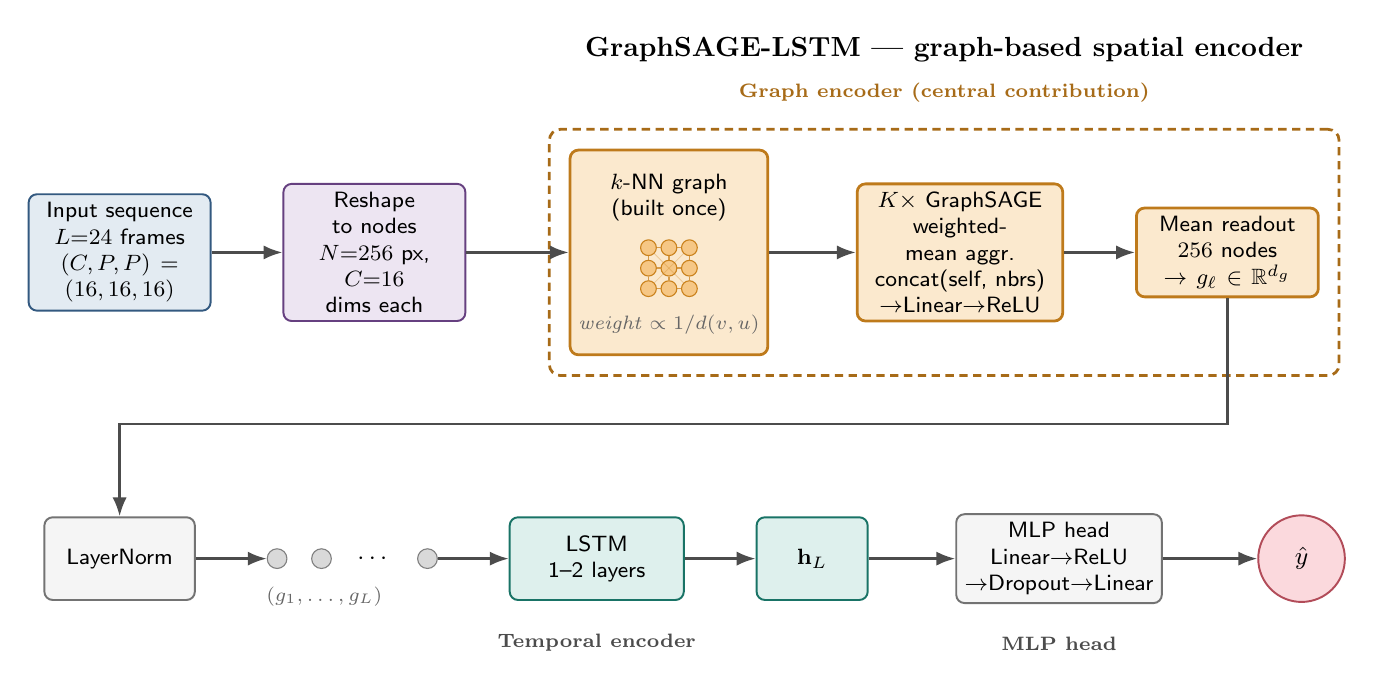
\begin{tikzpicture}[node distance=7mm]

  % ----------------------------------------------------------------
  % Row 1 (top): spatial path  —  Input -> reshape -> graph encoder
  % ----------------------------------------------------------------
  \node[inputblock] (input)
    {Input sequence\\ $L{=}24$ frames\\ \footnotesize $(C,P,P)=(16,16,16)$};

  \node[spatialblock, right=9mm of input, text width=2.1cm] (reshape)
    {Reshape to nodes\\ \footnotesize $N{=}256$ px,\\ $C{=}16$ dims each};

  % --- k-NN graph inset: pixel grid on top, weight caption BELOW the box
  %     (kept clear of the grid so nothing overlaps) ---
  \node[graphblock, right=13mm of reshape, text width=2.3cm, minimum height=2.6cm] (graphbox)
    {};
  \node[font=\sffamily\footnotesize, align=center, anchor=north, yshift=-2mm] at (graphbox.north)
    {$k$-NN graph\\ (built once)};

  \begin{scope}[shift={($(graphbox.center)+(0,-2mm)$)}]
    \foreach \i in {0,1,2} {
      \foreach \j in {0,1,2} {
        \node[pixnode] (px-\i-\j) at (\i*2.6mm-2.6mm, \j*2.6mm-2.6mm) {};
      }
    }
    \foreach \i in {0,1,2} {
      \foreach \j [remember=\j as \jlast (initially 0)] in {1,2} {
        \draw[cGraph!85!black, line width=0.5pt, opacity=0.75] (px-\i-\jlast) -- (px-\i-\j);
      }
    }
    \foreach \j in {0,1,2} {
      \foreach \i [remember=\i as \ilast (initially 0)] in {1,2} {
        \draw[cGraph!85!black, line width=0.5pt, opacity=0.75] (px-\ilast-\j) -- (px-\i-\j);
      }
    }
    \draw[cGraph!85!black, line width=0.3pt, opacity=0.30] (px-0-0) -- (px-2-2);
    \draw[cGraph!85!black, line width=0.3pt, opacity=0.30] (px-0-2) -- (px-2-0);
  \end{scope}
  \node[dimlabel, anchor=south, yshift=1.5mm] at (graphbox.south)
    {weight $\propto 1/d(v,u)$};

  \node[graphblock, right=11mm of graphbox, text width=2.4cm] (sage)
    {$K\times$ GraphSAGE\\ \footnotesize weighted-mean aggr.\\
     concat(self, nbrs)\\ $\to$Linear$\to$ReLU};

  \node[graphblock, right=9mm of sage, text width=2.1cm] (readout)
    {Mean readout\\ \footnotesize $256$ nodes\\ $\to g_\ell \in \mathbb{R}^{d_g}$};

  \node[graphgroupbox, fit=(graphbox)(sage)(readout)] (gbox) {};
  \node[grouplabel, text=cGraph!70!black, above=2mm of gbox.north]
    {Graph encoder (central contribution)};

  % ----------------------------------------------------------------
  % Row 2 (bottom): temporal path
  %   LayerNorm -> sequence -> LSTM -> h_L -> MLP head -> y
  %   Pushed down enough that its group labels (placed BELOW the row)
  %   never come near the graph encoder box above.
  % ----------------------------------------------------------------
  \node[neutralblock, below=26mm of input, text width=1.7cm] (ln) {LayerNorm};

  \node[seqdot, right=9mm of ln]                  (s1) {};
  \node[seqdot, right=3mm of s1]                  (s2) {};
  \node[font=\small, right=2mm of s2]             (sdots) {$\cdots$};
  \node[seqdot, right=2mm of sdots]               (sL) {};
  \node[dimlabel, below=1mm of s1, xshift=6mm] {$(g_1,\dots,g_L)$};

  \node[temporalblock, right=9mm of sL, text width=2.0cm] (lstm)
    {LSTM\\ \footnotesize 1--2 layers};

  \node[temporalblock, right=9mm of lstm, text width=1.2cm] (hL) {$\mathbf{h}_L$};

  \node[headblock, right=11mm of hL] (mlphead)
    {MLP head\\ \footnotesize Linear$\to$ReLU\\ $\to$Dropout$\to$Linear};

  \node[outputblock, right=12mm of mlphead] (out) {$\hat{y}$};

  \node[grouplabel, below=3mm of lstm] {Temporal encoder};
  \node[grouplabel, below=3mm of mlphead] {MLP head};

  % ----------------------------------------------------------------
  % Arrows
  % ----------------------------------------------------------------
  \draw[flow] (input) -- (reshape);
  \draw[flow] (reshape) -- (graphbox);
  \draw[flow] (graphbox) -- (sage);
  \draw[flow] (sage) -- (readout);
  \draw[flow] (readout.south) |- ($(gbox.south)+(0,-6mm)$) -| (ln.north);
  \draw[flow] (ln) -- (s1);
  \draw[flow] (sL) -- (lstm);
  \draw[flow] (lstm) -- (hL);
  \draw[flow] (hL) -- (mlphead);
  \draw[flow] (mlphead) -- (out);

  % ----------------------------------------------------------------
  % Title
  % ----------------------------------------------------------------
  \node[font=\bfseries\normalsize] at ($(gbox.north)+(0,10mm)$)
    {GraphSAGE-LSTM --- graph-based spatial encoder};

\end{tikzpicture}
\end{document}
